%Dạng 1
\setcounter{ex}{0}
\section{Bài toán liên quan đến giao điểm giữa các đồ thị}
\subsection{Kiến thức cần nhớ}
\begin{khung}
	\subsubsection{Số giao điểm của hai đồ thị}
	\begin{itemize}
		\item Muốn tìm số giao điểm giữa đồ thị hàm $y=f(x)$ và đường thẳng $y=a$ ta chỉ việc vẽ đường thẳng $y=a$ (là đường thẳng song song với trục $Ox$ và đi qua điểm có tọa độ $(0;a)$) và xác định số giao điểm.
		\item  Chú ý: Phương trình của trục hoành (hay trục $Ox$) là $y=0$.
		\item Cho hai hàm số $y=f(x)$ và $y=g(x)$, khi đó số giao điểm giữa hai đồ thị hàm số trên bằng số nghiệm của phương trình hoành độ giao điểm $f(x)=g(x)$.
		\item Trường hợp đề cho bảng biến thiên của hàm $y=f(x)$, để biểu diễn đường $y=a$ ta vẽ một đường ngang sao cho hợp lí với đề bài.
			\end{itemize}
			\subsubsection{Tìm giao điểm của hai đồ thị}
			\begin{itemize}
				\item Dựa vào đồ thị để tìm tạo độ giao điểm.\item Tìm nghiệm của phương trình hoành độ giao điểm, ta được hoành độ của giao điểm sau đó thay vào hàm số để tìm tung độ. \item Muốn tìm nghiệm của phương trình $f(u(x))=a$, ta đi giải phương trình $u(x)=x_0$ (trong đó $x_0$ là nghiệm của phương trình $f(x)=a$).
			\end{itemize}
\end{khung}
\subsection{Bài tập mẫu}
\Opensolutionfile{ans}[ans/ANS-cau-7]
\begin{khung}
	\begin{vd}[Đề tham khảo BGD 2023]%[2D1Y5-3]
		\immini{Cho hàm số $f(x) = \dfrac{ax+b}{cx+d}$ có đồ thị là đường cong trong hình bên. Tọa độ giao điểm của đồ thị hàm số với trục hoành là
			\choice
			{$(0;-2)$} {\True $(2;0)$} {$(-2;0)$} {$(0;2)$}}{
			\begin{tikzpicture}[>=stealth,line join=round,line cap=round,font=\footnotesize,scale=0.5]
				
				\def\a{1}
				\def\b{-2}
				\def\c{1}
				\def\d{1}
				\draw[->] (-5,0) -- (5,0) node[below] {\scriptsize $x$};
				\draw[->] (0,-3) -- (0,5) node[left] {\scriptsize $y$};
				\draw (0,1) node [above left] {$1$};
				\draw (-1,0) node [below left] {$-1$};
				\draw (0,-2) node [left] {$-2$};
				\draw (0,0)node[below right]{\footnotesize $O$} (2,0)node[below right]{$2$};
				\draw[dashed] (-1,-3)--(-1,5) (-5,1)--(5,1); % Vẽ TCĐ và TCN
				\clip (-5,-3)rectangle(5,5);
				\draw[fill] (0,0) circle(1pt);
				\pgfmathsetmacro{\can}{-(\d)/(\c)}
				\draw[thick,samples=150,smooth,domain=-5:{\can-.1}] plot(\x,{(\a*\x+(\b))/(\c*\x+(\d))}); % Vẽ nhánh bên trái TCĐ
				\draw[thick,samples=150,smooth,domain={\can+.1}:5] plot(\x,{(\a*\x+(\b))/(\c*\x+(\d))}); % Vẽ nhánh bên phải TCĐ
		\end{tikzpicture}}
		\loigiai{
			Nhìn vào hình trên ta thấy tạo độ giao điểm là $(2;0)$.}
	\end{vd}
\end{khung}
\subsection{Bài tập tương tự và phát triển}
\begin{ex}%[2D1B5-4] 
	\immini{
		Cho hàm số $f(x)= ax^3 +bx^2 +cx+d$ có đồ thị như hình bên. Phương trình $3f(x)+4=0$ có tất cả bao nhiêu nghiệm?
		\choice
		{\True $3$}
		{$0$}
		{$1$}
		{$2$}}{\begin{tikzpicture}[scale=0.8, font=\footnotesize, line join=round, line cap=round, >=stealth]
		\def\xmin{-2}\def\xmax{4}\def\ymin{-3}\def\ymax{3}
		\draw[->] (\xmin-0.2,0)--(\xmax+0.2,0) node[below] {\footnotesize $x$};
		\draw[->] (0,\ymin-0.2)--(0,\ymax+0.2) node[right] {\footnotesize $y$};
		\draw (0,0) node [below left] {\footnotesize $O$};
		\foreach \x in {2}\draw (\x,-0.1)--(\x,0.1) node [above] {\footnotesize $\x$};
		\foreach \y in {-2,2}\draw (0.1,\y)--(-0.1,\y) node [left] {\footnotesize $\y$};
		\clip (\xmin,\ymin) rectangle (\xmax,\ymax);
		\draw[smooth,samples=200,domain=\xmin:\xmax] plot (\x,{1*((\x)^3)+-3*((\x)^2)+0*(\x)+2});
		\draw[dashed] (2.0,0)--(2.0,-2.0)--(0,-2.0);
\end{tikzpicture}} 
\loigiai{\begin{center}
		\begin{tikzpicture}[scale=0.8, font=\footnotesize, line join=round, line cap=round, >=stealth]
			\def\xmin{-2}\def\xmax{4}\def\ymin{-3}\def\ymax{3}
			\draw[->] (\xmin-0.2,0)--(\xmax+0.2,0) node[below] {\footnotesize $x$};
			\draw[->] (0,\ymin-0.2)--(0,\ymax+0.2) node[right] {\footnotesize $y$};
			\draw (0,0) node [below left] {\footnotesize $O$};
			\foreach \x in {2}\draw (\x,-0.1)--(\x,0.1) node [above] {\footnotesize $\x$};
			\foreach \y in {-2,2}\draw (0.1,\y)--(-0.1,\y) node [left] {\footnotesize $\y$};
			\clip (\xmin,\ymin) rectangle (\xmax,\ymax);
			\draw[smooth,samples=200,domain=\xmin:\xmax] plot (\x,{1*((\x)^3)+-3*((\x)^2)+0*(\x)+2});
			\draw[dashed] (2.0,0)--(2.0,-2.0)--(0,-2.0);
			\draw[thick,samples=150,smooth,domain=-3.8:5.7,color=blue] plot(\x,-4/3); % Vẽ nhánh bên phải TCĐ
			\draw[color=blue] (3.2,-4/3) node [below] {$y=-\dfrac{4}{3}$};
		\end{tikzpicture}
	\end{center}
Ta có	$3f(x)+4=0 \Leftrightarrow f(x)=-\dfrac{4}{3}.$
	\\ Số nghiệm của phương trình là số giao điểm của $(C) \colon y=f(x)$ (hình vẽ) và $d \colon y=-\dfrac{4}{3}.$\\Vậy phương trình có 3 nghiệm.
}\end{ex}
\begin{ex}%[2D1B5-4]
	\immini{
	Cho hàm số $f(x) = ax^3 + bx^2 +cx+d$ có đồ thị như hình bên. Phương trình $2f(x)-5=0$ có tất cả bao nhiêu nghiệm?
	\choice
	{$3$}
	{$0$}
	{\True $1$}
	{$2$}}{\begin{tikzpicture}[scale=0.8, font=\footnotesize, line join=round, line cap=round, >=stealth]
	\def\xmin{-2}\def\xmax{4}\def\ymin{-3}\def\ymax{3}
	\draw[->] (\xmin-0.2,0)--(\xmax+0.2,0) node[below] {\footnotesize $x$};
	\draw[->] (0,\ymin-0.2)--(0,\ymax+0.2) node[right] {\footnotesize $y$};
	\draw (0,0) node [below left] {\footnotesize $O$};
	\foreach \x in {2}\draw (\x,-0.1)--(\x,0.1) node [above] {\footnotesize $\x$};
	\foreach \y in {-2,2}\draw (0.1,\y)--(-0.1,\y) node [left] {\footnotesize $\y$};
	\clip (\xmin,\ymin) rectangle (\xmax,\ymax);
	\draw[smooth,samples=200,domain=\xmin:\xmax] plot (\x,{1*((\x)^3)+-3*((\x)^2)+0*(\x)+2});
	\draw[dashed] (2.0,0)--(2.0,-2.0)--(0,-2.0);
\end{tikzpicture}} 
\loigiai{\begin{center}
		\begin{tikzpicture}[scale=0.8, font=\footnotesize, line join=round, line cap=round, >=stealth]
			\def\xmin{-2}\def\xmax{4}\def\ymin{-3}\def\ymax{3}
			\draw[->] (\xmin-0.2,0)--(\xmax+0.2,0) node[below] {\footnotesize $x$};
			\draw[->] (0,\ymin-0.2)--(0,\ymax+0.2) node[right] {\footnotesize $y$};
			\draw (0,0) node [below left] {\footnotesize $O$};
			\foreach \x in {2}\draw (\x,-0.1)--(\x,0.1) node [above] {\footnotesize $\x$};
			\foreach \y in {-2,2}\draw (0.1,\y)--(-0.1,\y) node [left] {\footnotesize $\y$};
			\clip (\xmin,\ymin) rectangle (\xmax,\ymax);
			\draw[smooth,samples=200,domain=\xmin:\xmax] plot (\x,{1*((\x)^3)+-3*((\x)^2)+0*(\x)+2});
			\draw[dashed] (2.0,0)--(2.0,-2.0)--(0,-2.0);
			\draw[thick,samples=150,smooth,domain=-4:5.7,color=blue] plot(\x,5/2); % Vẽ nhánh bên phải TCĐ
			\draw[color=blue] (3.2,5/2) node [below] {$y=\dfrac{5}{2}$};
		\end{tikzpicture}
	\end{center}
Ta có $2f(x)-5=0 \Leftrightarrow f(x)=\dfrac{5}{2}.$
\\ Số nghiệm của phương trình là số giao điểm của $(C) \colon y=f(x)$ (hình vẽ) và $d \colon y=\dfrac{5}{2}.$\\Vậy phương trình có 1 nghiệm.
} \end{ex}
\begin{ex}%[2D1B5-4]
	\immini{
	Cho hàm số $f(x) = ax^4 +bx^2+c$ có đồ thị như hình bên. Số nghiệm thực của phương trình $4f(x)-3=0$ là
	\choice
	{\True $4$}
	{$3$}
	{$2$}
	{$0$}}{\begin{tikzpicture}[scale=1, font=\footnotesize, line join=round, line cap=round, >=stealth]
	\def\xmin{-2.5}\def\xmax{2.5}\def\ymin{-1.5}\def\ymax{2}
	\draw[->] (\xmin-0.2,0)--(\xmax+0.2,0) node[below] {\footnotesize $x$};
	\draw[->] (0,\ymin-0.2)--(0,\ymax+0.2) node[right] {\footnotesize $y$};
	\draw (0,0) node [below left] {\footnotesize $O$};
	\foreach \x in {-1,1}\draw (\x,0.1)--(\x,-0.1) node [below] {\footnotesize $\x$};
	\foreach \y in {1}\draw (0.1,\y)--(-0.1,\y) node [above left] {\footnotesize $\y$};
	\clip (\xmin,\ymin) rectangle (\xmax,\ymax);
	\draw[smooth,samples=200,domain=\xmin:\xmax] plot (\x,{-1*((\x)^4)+2*((\x)^2)});
	\draw[dashed] (1.0,0)--(1.0,1.0)--(0,1.0);
	\draw[dashed] (-1.0,0)--(-1.0,1.0)--(0,1.0);
\end{tikzpicture}} 
\loigiai{
	\begin{center}
		\begin{tikzpicture}[scale=1, font=\footnotesize, line join=round, line cap=round, >=stealth]
			\def\xmin{-2.5}\def\xmax{2.5}\def\ymin{-1.5}\def\ymax{2}
			\draw[->] (\xmin-0.2,0)--(\xmax+0.2,0) node[below] {\footnotesize $x$};
			\draw[->] (0,\ymin-0.2)--(0,\ymax+0.2) node[right] {\footnotesize $y$};
			\draw (0,0) node [below left] {\footnotesize $O$};
			\foreach \x in {-1,1}\draw (\x,0.1)--(\x,-0.1) node [below] {\footnotesize $\x$};
			\foreach \y in {1}\draw (0.1,\y)--(-0.1,\y) node [above left] {\footnotesize $\y$};
			\clip (\xmin,\ymin) rectangle (\xmax,\ymax);
			\draw[smooth,samples=200,domain=\xmin:\xmax] plot (\x,{-1*((\x)^4)+2*((\x)^2)});
			\draw[dashed] (1.0,0)--(1.0,1.0)--(0,1.0);
			\draw[dashed] (-1.0,0)--(-1.0,1.0)--(0,1.0);	\draw[thick,samples=150,smooth,domain=-4:5.7,color=blue] plot(\x,3/4); % Vẽ nhánh bên phải TCĐ
			\draw[color=blue] (2,3/4) node [above] {$y=\dfrac{3}{4}$};
		\end{tikzpicture}
	\end{center}
Ta có $4f(x)-3=0 \Leftrightarrow f(x)=\dfrac{3}{4}.$
\\ Số nghiệm của phương trình là số giao điểm của $(C) \colon y=f(x)$ (hình vẽ) và $d \colon y=\dfrac{3}{4}.$\\Vậy phương trình có 4 nghiệm.
} \end{ex}
\begin{ex}%[2D1K5-4]
\immini{
		Cho hàm số $f(x)= ax^3+ bx^2 +cx+d$ có đồ thị như hình bên. Số nghiệm thực của phương trình $f(x^2)= -2$ là
		\choice 
		{$3$}
		{$4$}
		{$0$}
		{\True $2$}}{\begin{tikzpicture}[ font=\footnotesize, line join=round, line cap=round, >=stealth]
		\def\xmin{-2}\def\xmax{4}\def\ymin{-3}\def\ymax{3}
		\draw[->] (\xmin-0.2,0)--(\xmax+0.2,0) node[below] {\footnotesize $x$};
		\draw[->] (0,\ymin-0.2)--(0,\ymax+0.2) node[right] {\footnotesize $y$};
		\draw (0,0) node [below left] {\footnotesize $O$};
		\foreach \x in {1,2}\draw (\x,-0.1)--(\x,0.1) node [above] {\footnotesize $\x$};
		\foreach \y in {-2,2}\draw (0.1,\y)--(-0.1,\y) node [left] {\footnotesize $\y$};
		\clip (\xmin,\ymin) rectangle (\xmax,\ymax);
		\draw[smooth,samples=200,domain=\xmin:\xmax] plot (\x,{1*((\x)^3)+-3*((\x)^2)+0*(\x)+2});
		\draw[dashed] (2.0,0)--(2.0,-2.0)--(0,-2.0);
\end{tikzpicture}} 
\loigiai{\begin{center}
		\begin{tikzpicture}[font=\footnotesize, line join=round, line cap=round, >=stealth]
			\def\xmin{-2}\def\xmax{4}\def\ymin{-3}\def\ymax{3}
			\draw[->] (\xmin-0.2,0)--(\xmax+0.2,0) node[below] {\footnotesize $x$};
			\draw[->] (0,\ymin-0.2)--(0,\ymax+0.2) node[right] {\footnotesize $y$};
			\draw (0,0) node [below left] {\footnotesize $O$};
			\foreach \x in {1,2}\draw (\x,-0.1)--(\x,0.1) node [above] {\footnotesize $\x$};
			\foreach \y in {-2,2}\draw (0.1,\y)--(-0.1,\y) node [above left] {\footnotesize $\y$};
			\clip (\xmin,\ymin) rectangle (\xmax,\ymax);
			\draw[smooth,samples=200,domain=\xmin:\xmax] plot (\x,{1*((\x)^3)+-3*((\x)^2)+0*(\x)+2});
			\draw[dashed] (2.0,0)--(2.0,-2.0)--(0,-2.0);
			\draw[thick,samples=150,smooth,domain=-4:5.7,color=blue] plot(\x,-2);
		\end{tikzpicture}
	\end{center}
	Nhìn đồ thị ta thấy $f(x^2)= -2\Leftrightarrow \hoac{&x^2=x_0<0\\&x^2=2}\Leftrightarrow x=\pm \sqrt{2}.$
	\\ Vậy phương trình có 2 nghiệm thực phân biệt.
} \end{ex}
\begin{ex}%[2D1K5-4]
\immini{
		Cho hàm số $f(x)= ax^3+ bx^2 +cx+d$ có đồ thị như hình bên. Phương trình $f(x^2-2)=3$ có tất cả bao nhiêu nghiệm?
		\choice {$3$}
		{$2$}
		{$1$}
		{\True $4$}}{\begin{tikzpicture}[scale=.8, font=\footnotesize, line join=round, line cap=round, >=stealth]
		\def\xmin{-3}\def\xmax{3}\def\ymin{-2}\def\ymax{4}
		\draw[->] (\xmin-0.2,0)--(\xmax+0.2,0) node[below] {\footnotesize $x$};
		\draw[->] (0,\ymin-0.2)--(0,\ymax+0.2) node[right] {\footnotesize $y$};
		\draw (0,0) node [below left] {\footnotesize $O$};
		\foreach \x in {-1,2}\draw (\x,0.1)--(\x,-0.1) node [below] {\footnotesize $\x$};
		\foreach \x in {1}\draw (\x,-0.1)--(\x,0.1) node [above] {\footnotesize $\x$};
		\foreach \x in {-2}\draw (\x,-0.1)--(\x,0.1) node [above left] {\footnotesize $\x$};
		\foreach \y in {-1,1}\draw (0.1,\y)--(-0.1,\y) node [left] {\footnotesize $\y$};
		\foreach \y in {3}\draw (0.1,\y)--(-0.1,\y) node [above left] {\footnotesize $\y$};
		\clip (\xmin,\ymin) rectangle (\xmax,\ymax);
		\draw[smooth,samples=200,domain=\xmin:\xmax] plot (\x,{1*((\x)^3)+0*((\x)^2)+-3*(\x)+1});
		\draw[dashed] (0.0,0)--(0.0,1.0)--(0,1.0);\fill (0.0,1.0) circle (1pt);
		\draw[dashed] (-1.0,0)--(-1.0,3.0)--(0,3.0);
		\draw[dashed] (1.0,0)--(1.0,-1.0)--(0,-1.0);
		\draw[dashed] (2,0)--(2,3)--(0,3);
\end{tikzpicture}} 
\loigiai{\begin{center}
		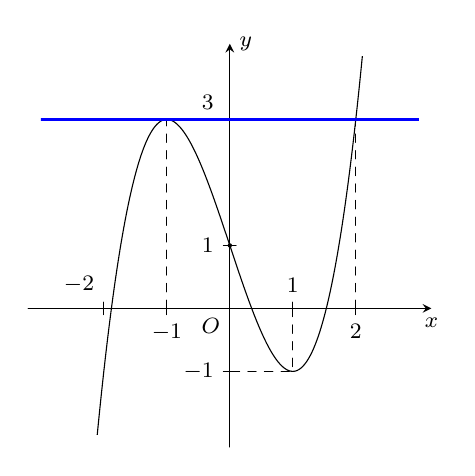
\begin{tikzpicture}[scale=.8, font=\footnotesize, line join=round, line cap=round, >=stealth]
			\def\xmin{-3}\def\xmax{3}\def\ymin{-2}\def\ymax{4}
			\draw[->] (\xmin-0.2,0)--(\xmax+0.2,0) node[below] {\footnotesize $x$};
			\draw[->] (0,\ymin-0.2)--(0,\ymax+0.2) node[right] {\footnotesize $y$};
			\draw (0,0) node [below left] {\footnotesize $O$};
			\foreach \x in {-1,2}\draw (\x,0.1)--(\x,-0.1) node [below] {\footnotesize $\x$};
			\foreach \x in {1}\draw (\x,-0.1)--(\x,0.1) node [above] {\footnotesize $\x$};
			\foreach \x in {-2}\draw (\x,-0.1)--(\x,0.1) node [above left] {\footnotesize $\x$};
			\foreach \y in {-1,1}\draw (0.1,\y)--(-0.1,\y) node [left] {\footnotesize $\y$};
			\foreach \y in {3}\draw (0.1,\y)--(-0.1,\y) node [above left] {\footnotesize $\y$};
			\clip (\xmin,\ymin) rectangle (\xmax,\ymax);
			\draw[smooth,samples=200,domain=\xmin:\xmax] plot (\x,{1*((\x)^3)+0*((\x)^2)+-3*(\x)+1});
			\draw[dashed] (0.0,0)--(0.0,1.0)--(0,1.0);\fill (0.0,1.0) circle (1pt);
			\draw[dashed] (-1.0,0)--(-1.0,3.0)--(0,3.0);
			\draw[dashed] (1.0,0)--(1.0,-1.0)--(0,-1.0);
			\draw[dashed] (2,0)--(2,3)--(0,3);
				\draw[thick,samples=150,smooth,domain=-4:5.7,color=blue] plot(\x,3);
		\end{tikzpicture}
	\end{center}
	Nhìn đồ thị ta thấy $f(x^2-2)=3\Leftrightarrow \hoac{&x^2-2=-1\\&x^2-2=2}\Leftrightarrow \hoac{&x=\pm 1\\&x=\pm 2.}$
	\\ Vậy phương trình có 4 nghiệm phân biệt.
} \end{ex}
\begin{ex} %[2D1B5-3]
	Cho hàm số $y=f(x)$ có bảng biến thiên như hình vẽ. 
	\begin{center}
		
\begin{tikzpicture}
			\tkzTabInit[nocadre,espcl=2.5,lgt=1.5]
			{$x$/0.7,$y'$/0.7,$y$/2.2}
			{$-\infty$,$-2$,$0$,$2$,$+\infty$}
			\tkzTabLine{,-,0,+,0,-,0,+}
			\tkzTabVar{+/$+\infty$,-/$-2$,+/$1$,-/$-2$,+/$+\infty$}\end{tikzpicture}
		\par\end{center}
	Số nghiệm của phương trình $2f(x)+3=0$ là 
	\choice 
	{\True $4$}{$3$} {$2$} {$1$} 
	\loigiai{ 
		Ta có $2f(x)+3=0\Leftrightarrow f(x)=-\dfrac{3}{2}$.
		$\hfill$ ({*}) \\
		Số nghiệm phương trình ({*}) là số giao điểm của đồ thị hàm số $y=f(x)$
		và đường thẳng $y=-\dfrac{3}{2}$. \\
		Bảng biến thiên.
		\begin{center}
			\begin{tikzpicture}
				\tkzTabInit[nocadre,espcl=2.5,lgt=1.5]
				{$x$/0.7,$y'$/0.7,$y$/3}
				{$-\infty$,$-2$,$0$,$2$,$+\infty$}
				\tkzTabLine{,-,z,+,0,-,z,+}
				\draw [-stealth] ($ (N12) -(0,0.5)$) node [above] {$ +\infty $}--($ (N23) + (-0.3,0.3) $) ;
				\draw ($ (N23) $) node  {$ -2 $};
				\draw [-stealth] ($ (N23) + (0.3,0.3) $) --($ (N32) + (-0.3,-1.8) $) ;
				\draw ($ (N32) + (0,-1.8) $) node  {$ 1 $};
				\draw ($ (N32) + (0.3,-1.8) $) -- ($ (N43) + (-0.3,0.3) $);
				\draw [-stealth] ($ (N43) + (0.3,0.3) $)  -- ($ (N52) -(0,0.5)$) node [above] {$ +\infty $};
				\draw ($ (N43) + (0,0.3) $)  node [below]  {$ -2 $};
				\draw [color=blue] ($ (N12) + (0,-2.2)$) --($ (N52) + (0,-2.2) $) node [below] {$ y=-\dfrac{3}{2} $} ;
			\end{tikzpicture}
			\par\end{center}
		\noindent Dựa vào bảng biến thiên ta được phương trình $f(x)=-\dfrac{3}{2}$
		có bốn nghiệm phân biệt.
} \end{ex}

\begin{ex} %[2D1B5-3]
	Cho hàm số $y=f(x)$ có bảng biến thiên như hình vẽ.
	\begin{center}
		
\begin{tikzpicture}
			\tkzTabInit[nocadre,espcl=2.5,lgt=1.5]
			{$x$/0.6,$y'$/0.6,$y$/2.2}
			{$-\infty$,$-2$,$3$,$+\infty$}
			\tkzTabLine{,+,d,-,d,+,}
			\tkzTabVar{-/$-\infty$,+/$2$,-/$1$,+/$+\infty$}\end{tikzpicture}
		\par\end{center}
	Số nghiệm thực của phương trình $2f(x)-3=0$ là 
	\choice {$2$}{$1$} {\True $3$ } {$4$ } 
	\loigiai{Ta có $2f(x)-3=0\Leftrightarrow f(x)=\dfrac{3}{2}.$
		$\hfill(*)$ \\
		Số nghiệm phương trình ({*}) là số giao điểm của đồ thị hàm số $y=f(x)$
		và đường thẳng $y=\dfrac{3}{2}$. \\
		Bảng biến thiên.
		\begin{center}
			\begin{tikzpicture}
				\tkzTabInit[nocadre,espcl=2.5,lgt=1.5]
				{$x$/0.6,$y'$/0.6,$y$/2.2}
				{$-\infty$,$-2$,$3$,$+\infty$}
				\tkzTabLine{,+,d,-,d,+,}
				\tkzTabVar{-/$-\infty$,+/$2$,-/$1$,+/$+\infty$}
				\draw [color=blue] ($(N13)!0.5!(N12) $) -- ($ (N42)!0.5!(N43) $)  node [below] {$ y=\dfrac{3}{2} $};
			\end{tikzpicture}
			\par\end{center}
		\noindent Dựa vào bảng biến thiên ta được phương trình $f(x)=\dfrac{3}{2}$
		có ba nghiệm phân biệt. 
} \end{ex}
\begin{ex} %[2D1B5-3]
	Cho hàm số $y=f(x)$ có bảng biến thiên như hình vẽ.
	\begin{center}
		
\begin{tikzpicture}
			\tkzTabInit[nocadre,espcl=2.5,lgt=1.5]
			{$x$/0.7,$y'$/0.7,$y$/2.2}
			{$-\infty$,$-2$,$0$,$2$,$+\infty$}
			\tkzTabLine{,-,0,+,0,-,0,+}
			\tkzTabVar{+/$+\infty$,-/$-2$,+/$1$,-/$-2$,+/$+\infty$}
		\end{tikzpicture}
		\par\end{center}
	Số nghiệm của phương trình $2f(x)-3=0$ là 
	\choice {$4$} {$3$} {\True $2$ } {$1$} 
	\loigiai{Ta có phương trình $2f(x)-3=0\Leftrightarrow f(x)=\dfrac{3}{2}.\hfill(*)$
		\\
		Số nghiệm phương trình ({*}) là số giao điểm của đồ thị hàm số $y=f(x)$
		và đường thẳng $y=\dfrac{3}{2}$.\\
		Xét bảng biến thiên.
		\begin{center}
			\begin{tikzpicture}
				\tkzTabInit[nocadre,espcl=2.5,lgt=1.5]
				{$x$/0.7,$y'$/0.7,$y$/3}
				{$-\infty$,$-2$,$0$,$2$,$+\infty$}
				\tkzTabLine{,-,0,+,0,-,0,+}
				\draw [-stealth] ($ (N12) -(0,0.5)$) node [above] {$ +\infty $}--($ (N23) + (-0.3,0.3) $) ;
				\draw ($ (N23) $) node  {$ -2 $};
				\draw [-stealth] ($ (N23) + (0.3,0.3) $) --($ (N32) + (-0.3,-1.8) $) ;
				\draw ($ (N32) + (0,-1.8) $) node  {$ 1 $};
				\draw ($ (N32) + (0.3,-1.8) $) -- ($ (N43) + (-0.3,0.3) $);
				\draw [-stealth] ($ (N43) + (0.3,0.3) $)  -- ($ (N52) -(0,0.5)$) node [above] {$ +\infty $};
				\draw ($ (N43) + (0,0.3) $)  node [below]  {$ -2 $};
				\draw [color=blue] ($ (N12) + (0,-1.2)$) --($ (N52) + (0,-1.2) $) node [below] {$ y=\dfrac{3}{2} $} ;
			\end{tikzpicture}
			\par\end{center}
		\noindent Dựa vào bảng biến thiên ta được phương trình $f(x)=\dfrac{3}{2}$
		có hai nghiệm phân biệt.
} \end{ex}

\begin{ex} %[2D1B5-3]
	Cho hàm số $y=f(x)$ có bảng biến thiên nhu hình vẽ. 
	\begin{center}
		
\begin{tikzpicture}
			\tkzTabInit[nocadre,espcl=3.5,lgt=1.5]
			{$ x $/0.7,$ y' $/0.7,$ y $/2.5}
			{$ -\infty $,$ -1 $,$ 3 $,$ +\infty $}
			\tkzTabLine{,+, z ,-, z ,+,}
			\tkzTabVar{-/$ 2 $,+/$ 5 $,-/$ 1 $,+/$ +\infty $}
		\end{tikzpicture} 
		\par\end{center}
	Phương trình $f(x)-2=0$ có bao nhiêu nghiệm? 
	\choice { $1$} {$3$}{\True $2$} { $0$} 
	\loigiai{Ta có $f(x)-2=0\Leftrightarrow f(x)=2$.
		$\hfill(*)$\\
		Số nghiệm phương trình ({*}) là số giao điểm của đồ thị hàm số $y=f(x)$
		và đường thẳng $y=2$.\\
		Bảng biến thiên.
		\begin{center}
			\begin{tikzpicture}
				\tkzTabInit[nocadre,espcl=3.5,lgt=1.5]
				{$ x $/0.7,$ y' $/0.7,$ y $/3}
				{$ -\infty $,$ -1 $,$ 3 $,$ +\infty $}
				\tkzTabLine{,+, z ,-, z ,+,}
				\draw [-stealth] ($ (N13)+(0.2,1.5) $)--($ (N22)+(-0.2,-0.7) $);
				\draw [-stealth] ($ (N22)+(0.2,-0.7) $)--($ (N33)+(-0.2,0.2) $);
				\draw [-stealth] ($ (N33)+(0.2,0.2) $)--($ (N42)+(-0.2,-0.4) $);
				\draw [color=blue] ($ (N13)+(0.2,1.5) $)--($ (N43)+(0.2,1.5) $) node [below] {$ y=2 $};
				\draw ($ (N33)+(0,0.2) $) node [below] {$ 1 $};
				\draw  ($ (N13)+(0,1.5) $) node [below] {$ 2 $};
				\draw ($ (N22)+(0,-0.7) $) node  {$ 5 $};
				\draw ($ (N42)+(-0.2,-0.3) $) node  {$ +\infty $};\end{tikzpicture}
			\par\end{center}
		\noindent Ta có $\lim\limits _{x\to-\infty}f(x)=2$.\\
		Dựa vào bảng biến thiên ta được phương trình $f(x)=2$ có hai nghiệm
		phân biệt.
} \end{ex}
\begin{ex} %[2D1B5-3]
\immini{Cho hàm số $f(x) = \dfrac{ax+b}{cx+d}$ có đồ thị như hình bên. Tìm tọa độ giao điểm của đồ thị hàm số bên với đường thẳng $y =-1$.
	\choice
	{$(0;1)$} {\True $(0;-1)$} {$(-1;-1)$} {$(-1;0)$}}{
	\begin{tikzpicture}[>=stealth,line join=round,line cap=round,font=\footnotesize,scale=0.7]
		
		\def\a{1}
		\def\b{1}
		\def\c{1}
		\def\d{-1}
		\draw[->] (-3,0) -- (5,0) node[below] {\scriptsize $x$};
		\draw[->] (0,-3) -- (0,5) node[left] {\scriptsize $y$};
		\draw (0,1) node [above left] {$1$};
		\draw (-1,0) node [below left] {$-1$};
		\draw (0,-1) node [left] {$-1$};
		\draw (0,0)node[below right]{\footnotesize $O$} (1,0)node[below right]{$1$};
		\draw[dashed] (1,-3)--(1,5) (-3,1)--(5,1); % Vẽ TCĐ và TCN
		\clip (-3,-3)rectangle(5,5);
		\draw[fill] (0,0) circle(1pt);
		\pgfmathsetmacro{\can}{-(\d)/(\c)}
		\draw[thick,samples=150,smooth,domain=-3:{\can-.1}] plot(\x,{(\a*\x+(\b))/(\c*\x+(\d))}); % Vẽ nhánh bên trái TCĐ
		\draw[thick,samples=150,smooth,domain={\can+.1}:5] plot(\x,{(\a*\x+(\b))/(\c*\x+(\d))}); % Vẽ nhánh bên phải TCĐ
\end{tikzpicture}}
\loigiai{\begin{center}
	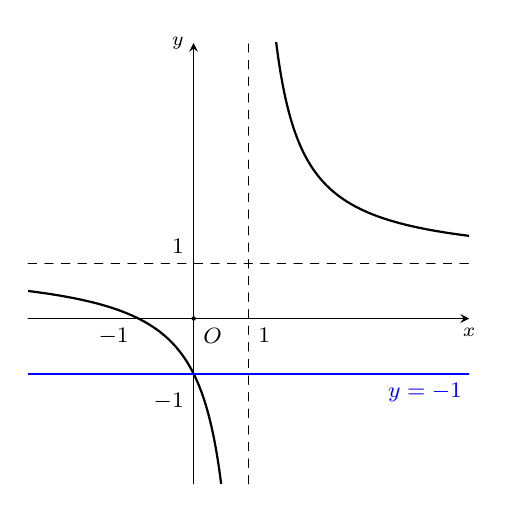
\begin{tikzpicture}[>=stealth,line join=round,line cap=round,font=\footnotesize,scale=0.7]
		
		\def\a{1}
		\def\b{1}
		\def\c{1}
		\def\d{-1}
		\draw[->] (-3,0) -- (5,0) node[below] {\scriptsize $x$};
		\draw[->] (0,-3) -- (0,5) node[left] {\scriptsize $y$};
		\draw (0,1) node [above left] {$1$};
		\draw (-1,0) node [below left] {$-1$};
		\draw (0,-1.5) node [left] {$-1$};
		\draw (0,0)node[below right]{\footnotesize $O$} (1,0)node[below right]{$1$};
		\draw[dashed] (1,-3)--(1,5) (-3,1)--(5,1); % Vẽ TCĐ và TCN
		\clip (-3,-3)rectangle(5,5);
		\draw[fill] (0,0) circle(1pt);
		\pgfmathsetmacro{\can}{-(\d)/(\c)}
		\draw[thick,samples=150,smooth,domain=-3:{\can-.1}] plot(\x,{(\a*\x+(\b))/(\c*\x+(\d))}); % Vẽ nhánh bên trái TCĐ
		\draw[thick,samples=150,smooth,domain={\can+.1}:5] plot(\x,{(\a*\x+(\b))/(\c*\x+(\d))});
		\draw[thick,samples=150,smooth,domain=-3:5,color=blue] plot(\x,-1); % Vẽ nhánh bên phải TCĐ
		\draw[color=blue] (4.2,-1) node [below] {$y=-1$};
	\end{tikzpicture}
	\end{center}
Nhìn vào hình trên ta thấy tọa độ giao điểm là $(0;-1)$.}
\end{ex}
\begin{ex}%[2D1B5-3]
Giao điểm của đồ thị hàm số $y=\dfrac{2 x+1}{x+1}$ với trục hoành là điểm
\choice{\True$N\left(-\dfrac{1}{2} ; 0\right)$}{$P\left(\dfrac{1}{2} ; 0\right)$}{$Q(-1 ; 0)$}{$M(0 ; 1)$}
\loigiai{Giao với trục $Oy$ cho $y=0 \Leftrightarrow \dfrac{2 x+1}{x+1}=0 \Leftrightarrow x=-\dfrac{1}{2}$.\\
	Vậy giao điểm của đồ thị hàm số với trục $O y$ là điểm $N\left(-\dfrac{1}{2} ; 0\right)$.}
\end{ex}
\begin{ex}%[2D1B5-3]
	Cho hàm số $y=x^3-3 x$ có đồ thị $(C)$. Tìm số giao điểm của $(C)$ và trục hoành.
	\choice{\True$3$}{$1$}{$0$}{$2$}
	\loigiai{Xét phương trình hoành độ giao điểm của $(C)$ và trục hoành: $x^3-3 x=0 \Leftrightarrow\hoac{&x=0 \\ &x= \pm \sqrt{3}.}$\\
		Vậy số giao điểm của $(C)$ và trục hoành là $3$.}
\end{ex}
\begin{ex}%[2D1B5-3]
Đồ thị hàm số $y=\left(x^2-1\right)\left(x^2+1\right)$ cắt trục hoành tại bao nhiêu điểm phân biệt?
	\choice{$1$}{\True$2$}{$0$}{$4$}
	\loigiai{Ta có $y=0 \Rightarrow x= \pm 1$. Do đó đồ thị cắt trục hoành tại 2 điểm phân biệt.}
\end{ex}
\begin{ex}%[2D1B5-3]
Đường thẳng $y=x-1$ cắt đồ thị hàm số $y=x^3-x^2+x-1$ tại hai điểm phân biệt. Tìm tổng tung độ các giao điểm đó.
	\choice{$2$}{\True$-1$}{$-3$}{$0$}
	\loigiai{Xét phương trình $x^3-x^2+x-1=x-1 \Leftrightarrow x^3-x^2=0 \Leftrightarrow x^2(x-1)=0 \Leftrightarrow\hoac{&x=0 \\& x=1.}$\\
		Với $x=0 \Rightarrow y=-1=y_1$.\\
		Với $x=1 \Rightarrow y=0=y_2$.\\
		Vậy tổng các tung độ của các giao điểm là $y_1+y_2=-1+0=-1$.}
\end{ex}
\begin{ex}%[2D1B5-3]
	Tính tổng hoành độ của các giao điểm của đồ thị hàm số $y=\dfrac{5 x+6}{x+2}$ và đường thẳng $y=-x$.
	\choice{$-5$}{\True$-7$}{$5$}{$7$}
	\loigiai{Xét phương trình hoành độ giao điểm: $\dfrac{5 x+6}{x+2}=-x\ ($ với $x \neq-2)$
		$$
		\Leftrightarrow 5 x+6=-x(x+2) \Leftrightarrow x^2+7 x+6=0 \Leftrightarrow\hoac{
			&x=-1 \\
			&x=-6.
		} $$
		Khi đó tổng hoành độ của các giao điểm là $-7$.}
\end{ex}
\begin{ex}%[2D1B5-3]
Đồ thị của hàm số $y=4 x^4-2 x^2+1$ và đồ thị của hàm số $y=x^2+x+1$ có tất cả bao nhiêu điểm chung?
	\choice{$4$}{$1$}{$2$}{\True$3$}
	\loigiai{Phương trình hoành độ giao điểm: $4 x^4-2 x^2+1=x^2+x+1 \Leftrightarrow 4 x^4-3 x^2-x=0 \Leftrightarrow\hoac{&x=0 \\ &x=1 \\ &x=\dfrac{-1}{2}.}$
		Vậy đồ thị hai hàm số có 3 điểm chung.}
\end{ex}
\begin{ex}%[2D1B5-3]
	Trong các điểm sau điểm nào là giao điểm của đồ thị hàm số $y=x+\dfrac{2}{x-1}$ và đường thẳng $y=2 x$.
	\choice{$(2 ; -4)$}{$(-2 ; -2)$}{$(-1 ; 2)$}{\True$(2 ; 4)$}
	\loigiai{Ta có phương trình hoành độ giao điểm của hai đồ thị: $$x+\dfrac{2}{x-1}=2 x \Leftrightarrow \dfrac{2}{x-1}=x \Leftrightarrow x^2-x-2=0 \Leftrightarrow\hoac{&x=-1 \\ &x=2.}$$\\
		Từ đó ta có 2 giao điểm là $A(-1 ;-2)$ và $B(2 ; 4)$.}
\end{ex}
\begin{ex} %[2D1K5-3]
	Cho hàm số $y=f(x)$ có bảng biến thiên như hình vẽ. 
	\begin{center}
		
\begin{tikzpicture}
			\tkzTabInit[nocadre,espcl=3.5,lgt=1.5]
			{$ x $/0.7,$ y' $/0.7,$ y $/2.5}
			{$ -\infty $,$ 0 $,$ 1 $,$ +\infty $}
			\tkzTabLine{,-, d ,+,z,-,}
			\tkzTabVar{-/$ -\infty $,+D+/$ 2 $/$ +\infty $,-/$-4 $,+/$ +\infty  $}
		\end{tikzpicture}
		\par\end{center}
	Tìm số nghiệm thực của phương trình $f(x)-1=0$? 
	\choice {\True $3$} {$1$}
	{$2$} {$0$}
	\loigiai{Số nghiệm phương trình
		$f(x)-1=0$ là số giao điểm của đồ thị hàm số $y=f(x)$ và đường thẳng
		$y=1$.\\
		Bảng biến thiên.\\
		\begin{center}
			\begin{tikzpicture}
				\tkzTabInit[nocadre,espcl=3.5,lgt=1.5]
				{$ x $/0.7,$ y' $/0.7,$ y $/2.5}
				{$ -\infty $,$ 0 $,$ 1 $,$ +\infty $}
				\tkzTabLine{,-, d ,+,z,-,}
				\draw ($ (N12)!0.8!(N13) $) node [below] {$ -\infty $} ($ (N22)!0.4!(N23) +(-0.4,0) $) node [above] {$ 2 $};
				\draw [-stealth] ($ (N12)!0.8!(N13) + (0.2,-0.1) $) -- ($ (N22)!0.4!(N23) + (-0.4,0.1)$);
				\draw ($ (N22)!0.1!(N23) +(0.4,-0.2) $) node [above] {$ +\infty $}  ($ (N32)!0.7!(N33) $) node [below] {$ -4 $};
				\draw [-stealth] ($ (N22)!0.1!(N23) +(0.5,-0.3) $) -- ($ (N32)!0.7!(N33) +(-0.2,0)$);
				\draw ($ (N42)!0.1!(N43) +(-0.2,-0.2) $) node [above] {$ +\infty $};
				\draw [-stealth] ($ (N32)!0.7!(N33) +(0.2,0) $)--($ (N42)!0.1!(N43) +(-0.2,-0.3) $);
				\draw [blue] ($ (N12)!0.5!(N13) $) -- ($ (N42)!0.5!(N43) $) node [below] {$ y=1 $};
				\draw [double] (N22)--(N23);
			\end{tikzpicture}
		\end{center}
		\noindent Dựa vào bảng biên thiên ta được kết quả là 3 nghiệm. 
} \end{ex}
\begin{ex}%[2D1K5-4]
	\immini{
		Cho hàm số $y = f(x)$ có đồ thị trong hình bên. Phương trình $f(x)-1=0$ có bao nhiêu nghiệm thực phân biệt nhỏ hơn 2?
		\choice
		{$1$}
		{\True $2$}
		{$3$}
		{$0$}}{\begin{tikzpicture}[scale=0.8, font=\footnotesize, line join=round, line cap=round, >=stealth]
		\def\xmin{-2}\def\xmax{4}\def\ymin{-3}\def\ymax{3}
		\draw[->] (\xmin-0.2,0)--(\xmax+0.2,0) node[below] {\footnotesize $x$};
		\draw[->] (0,\ymin-0.2)--(0,\ymax+0.2) node[right] {\footnotesize $y$};
		\draw (0,0) node [below left] {\footnotesize $O$};
		\foreach \x in {2}\draw (\x,0.1)--(\x,-0.1) node [below] {\footnotesize $\x$};
		\foreach \y in {-2,2}\draw (0.1,\y)--(-0.1,\y) node [left] {\footnotesize $\y$};
		\clip (\xmin,\ymin) rectangle (\xmax,\ymax);
		\draw[smooth,samples=200,domain=\xmin:\xmax] plot (\x,{-1*((\x)^3)+3*((\x)^2)+0*(\x)-2});
		\draw[dashed] (2.0,0)--(2.0,2.0)--(0,2.0);
\end{tikzpicture}}
\loigiai{\begin{center}
		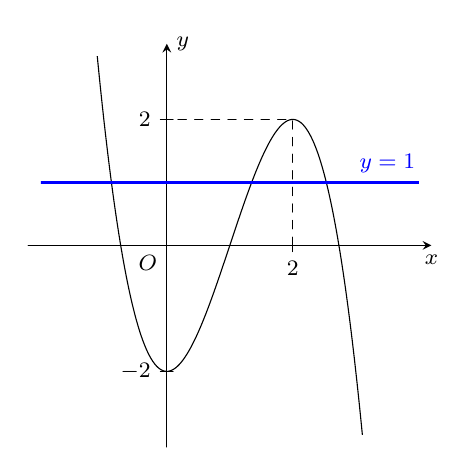
\begin{tikzpicture}[scale=0.8, font=\footnotesize, line join=round, line cap=round, >=stealth]
			\def\xmin{-2}\def\xmax{4}\def\ymin{-3}\def\ymax{3}
			\draw[->] (\xmin-0.2,0)--(\xmax+0.2,0) node[below] {\footnotesize $x$};
			\draw[->] (0,\ymin-0.2)--(0,\ymax+0.2) node[right] {\footnotesize $y$};
			\draw (0,0) node [below left] {\footnotesize $O$};
			\foreach \x in {2}\draw (\x,0.1)--(\x,-0.1) node [below] {\footnotesize $\x$};
			\foreach \y in {-2,2}\draw (0.1,\y)--(-0.1,\y) node [left] {\footnotesize $\y$};
			\clip (\xmin,\ymin) rectangle (\xmax,\ymax);
			\draw[smooth,samples=200,domain=\xmin:\xmax] plot (\x,{-1*((\x)^3)+3*((\x)^2)+0*(\x)-2});
			\draw[dashed] (2.0,0)--(2.0,2.0)--(0,2.0);
				\draw[thick,samples=150,smooth,domain=-4:5.7,color=blue] plot(\x,1);
			\draw[color=blue] (3.5,1) node [above] {$y=1$};
		\end{tikzpicture}
	\end{center}
Ta có	$f(x)-1=0 \Leftrightarrow f(x)=1.$
	\\ Số nghiệm của phương trình là số giao điểm của $(C) \colon y=f(x)$ (hình vẽ) và $d \colon y=1.$\\Vậy phương trình có 2 nghiệm thực phân biệt nhỏ hơn 2.
} \end{ex}
\begin{ex}%[2D1K5-4]
	\immini{
		Cho hàm số $f(x)= ax^3 + bx^2 + cx+d$ có đồ thị như hình bên. Phương trình $3f (x)-2 =0$ có bao nhiêu nghiệm lớn hơn 1?
		\choice
		{$3$}
		{$0$}
		{\True $1$}
		{$2$}}{\begin{tikzpicture}[scale=0.8, font=\footnotesize, line join=round, line cap=round, >=stealth]
		\def\xmin{-2}\def\xmax{4}\def\ymin{-3}\def\ymax{3}
		\draw[->] (\xmin-0.2,0)--(\xmax+0.2,0) node[below] {\footnotesize $x$};
		\draw[->] (0,\ymin-0.2)--(0,\ymax+0.2) node[right] {\footnotesize $y$};
		\draw (0,0) node [below left] {\footnotesize $O$};
		\foreach \x in {1,2}\draw (\x,-0.1)--(\x,0.1) node [above] {\footnotesize $\x$};
		\foreach \y in {-2,2}\draw (0.1,\y)--(-0.1,\y) node [left] {\footnotesize $\y$};
		\clip (\xmin,\ymin) rectangle (\xmax,\ymax);
		\draw[smooth,samples=200,domain=\xmin:\xmax] plot (\x,{1*((\x)^3)+-3*((\x)^2)+0*(\x)+2});
		\draw[dashed] (2.0,0)--(2.0,-2.0)--(0,-2.0);
\end{tikzpicture}} 
\loigiai{\begin{center}
		\begin{tikzpicture}[scale=0.8, font=\footnotesize, line join=round, line cap=round, >=stealth]
			\def\xmin{-2}\def\xmax{4}\def\ymin{-3}\def\ymax{3}
			\draw[->] (\xmin-0.2,0)--(\xmax+0.2,0) node[below] {\footnotesize $x$};
			\draw[->] (0,\ymin-0.2)--(0,\ymax+0.2) node[right] {\footnotesize $y$};
			\draw (0,0) node [below left] {\footnotesize $O$};
			\foreach \x in {1,2}\draw (\x,-0.1)--(\x,0.1) node [above] {\footnotesize $\x$};
			\foreach \y in {-2,2}\draw (0.1,\y)--(-0.1,\y) node [left] {\footnotesize $\y$};
			\clip (\xmin,\ymin) rectangle (\xmax+0.1,\ymax);
			\draw[smooth,samples=200,domain=\xmin:\xmax] plot (\x,{1*((\x)^3)+-3*((\x)^2)+0*(\x)+2});
			\draw[dashed] (2.0,0)--(2.0,-2.0)--(0,-2.0);
		\draw[thick,samples=150,smooth,domain=-4:5.7,color=blue] plot(\x,2/3);
		\draw[color=blue] (3.6,2/3) node [above] {$y=\dfrac{2}{3}$};
		\end{tikzpicture}
	\end{center}
Ta có	$3f (x)-2 =0 \Leftrightarrow f(x)=\dfrac{2}{3}.$
	\\ Số nghiệm của phương trình là số giao điểm của $(C) \colon y=f(x)$ (hình vẽ) và $d \colon y=\dfrac{2}{3}.$\\Vậy phương trình có 1 nghiệm lớn hơn 1.
} \end{ex}
\Closesolutionfile{ans}
%======================
\subsection{Bảng đáp án}
\inputansbox{8}{ans/ANS-cau-7}


